\documentclass[tikz,border=8pt]{standalone}
% Shared look for every TikZ diagram. Load with \input{../../tools/tikz-style.tex}
\usepackage[T1]{fontenc}
\usepackage{lmodern}
\renewcommand{\sfdefault}{lmr}  % diagrams use the same serif as the text
\usetikzlibrary{arrows.meta, positioning, shapes.geometric, calc, fit, backgrounds}
\definecolor{cblue}{HTML}{4C78A8}
\definecolor{corange}{HTML}{F58518}
\definecolor{cgreen}{HTML}{54A24B}
\definecolor{cred}{HTML}{E45756}
\definecolor{cpurple}{HTML}{B279A2}
\definecolor{cgrey}{HTML}{6B6B6B}
\tikzset{
  every picture/.style={font=\sffamily, line width=1.2pt},
  box/.style={draw=#1, fill=#1!12, rounded corners=4pt, align=center, inner sep=7pt, minimum height=1.1cm},
  box/.default=cgrey,
  arrow/.style={-{Stealth[length=3mm]}, draw=cgrey, line width=1.4pt},
  title/.style={font=\sffamily\bfseries\Large},
  note/.style={font=\sffamily\small, text=cgrey, align=center},
}
\AtBeginDocument{\hyphenpenalty=10000 \exhyphenpenalty=10000}

\begin{document}
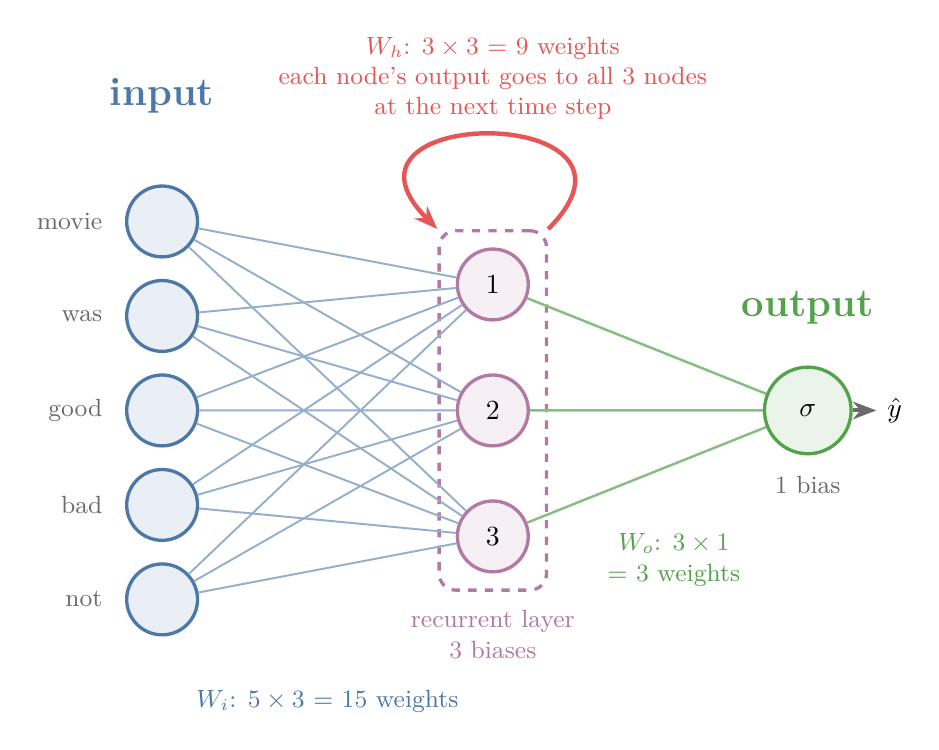
\begin{tikzpicture}[neuron/.style={circle, draw=#1, fill=#1!12, minimum size=0.9cm, line width=1.2pt}]
  \foreach \i/\w in {1/movie,2/was,3/good,4/bad,5/not} {
    \node[neuron=cblue] (x\i) at (0,-1.2*\i+3.6) {};
    \node[left=0.15cm of x\i, font=\sffamily\small, text=cgrey] {\w};
  }
  \foreach \j in {1,2,3} \node[neuron=cpurple] (h\j) at (4.2,-1.6*\j+3.2) {\j};
  \node[draw=cpurple, dashed, rounded corners=6pt, inner sep=6pt, fit=(h1)(h3)] (layer) {};
  \node[neuron=cgreen, minimum size=1.1cm] (y) at (8.2,0) {$\sigma$};
  \node[right=0.3cm of y] (yh) {$\hat{y}$};
  \draw[arrow] (y) -- (yh);
  \foreach \i in {1,...,5} \foreach \j in {1,2,3} \draw[cblue!60, line width=0.7pt] (x\i) -- (h\j);
  \foreach \j in {1,2,3} \draw[cgreen!70, line width=0.9pt] (h\j) -- (y);
  % feedback: the layer's 3 outputs return to all 3 nodes at the next time step
  \draw[cred, line width=1.6pt, -{Stealth[length=3mm]}] (layer.north east) .. controls +(1.6,1.6) and +(-1.6,1.6) .. (layer.north west);
  \node[note, text=cred, above=1.25cm of layer.north] {$W_h$: $3 \times 3$ = 9 weights\\each node's output goes to all 3 nodes\\at the next time step};
  \node[note, text=cblue] at (2.1,-3.7) {$W_i$: $5 \times 3$ = 15 weights};
  \node[note, text=cgreen] at (6.5,-1.9) {$W_o$: $3 \times 1$\\= 3 weights};
  \node[title, text=cblue] at (0,4.0) {input};
  \node[title, text=cgreen] at (8.2,1.3) {output};
  \node[note, text=cpurple, below=0.1cm of layer.south] {recurrent layer\\3 biases};
  \node[note] at (8.2,-0.95) {1 bias};
\end{tikzpicture}
\end{document}
